\chapter{Lo standard IEEE 802.21}

In questo capitolo sarà esposto lo standard IEEE 802.21\cite{ieee80221}, illustrandone le componenti e le loro funzionalità, al fine di avere un quadro completo e poter comprendere il suo reale obbiettivo, ovvero creare un meccanismo standardizzato per poter prendere più facilmente decisioni di {\em handover}, in modo che sia {\em media-independent}, ovvero indipendente dal mezzo trasmissivo utilizzato.

\section{Storia}
Con il continuo diffondersi di nuove tecnologie e dispositivi dotati di più interfacce di rete, è diventato necessario dover formalizzare alcune funzionalità per facilitare un passaggio indolore da una rete all'altra.
Come possiamo notare dalla figura \ref{fig:timeline}, il {\em working group} cominciò effettivamente i lavori nel marzo 2004 e la prima versione ufficiale dello standard fu pubblicata nel gennaio 2009. Gli eventi principali sono stati i seguenti:
\begin{itemize}
\item marzo 2003: creazione IEEE 802.21 ECSG\footnote{Executive Committee Study Group}
\item marzo 2004: creazione IEEE 802.21 WG\footnote{Working Group}
\item settembre 2004: analisi dei requisiti
\item ottobre 2004: raccolta delle proposte
\item maggio 2005: formulazione di una proposta unica
\item luglio 2005: inizio discussione della proposta
\item luglio 2007: IEEE 802 Sponsor Ballot\cite{balloting}
\item gennaio 2009: pubblicazione dello standard
\end{itemize}

\begin{figure}[h!]
\centering
\hspace*{-1em}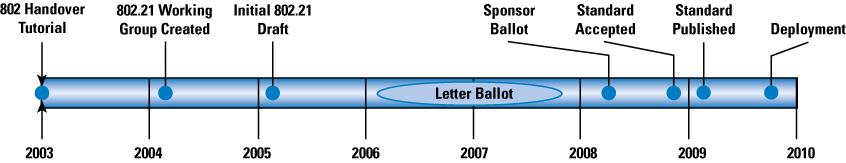
\includegraphics[scale=0.5]{ieee_timeline.jpg}
\caption{IEEE 802.21 Timeline}
\label{fig:timeline}
\end{figure}

\section{Finalità}
Lo standard IEEE 802.21 si pone l'obbiettivo di aiutare i nodi mobili a prepararsi ad eventuali azioni di {\em handover} da un {\em access point} all'altro, ma non specifica come debba avvenire la migrazione. Come sintetizzato dalla figura \ref{fig:rapporto}, esso si pone da intermediario tra gli standards coinvolti in azioni di {\em handover}: sono infatti definite tutte le funzionalità per acquisire informazioni sullo stato delle varie interfacce, ma non è specificato come e quando debba effettivamente avvenire l'eventuale passaggio, il quale ha bisogno di apposite specifiche. L'applicazione utente che usufruisce dei servizi offerti da questo standard è in grado di conoscere lo stato delle connessioni disponibili attraverso la ricezione di eventi dal proprio MIHF\footnote{Media Independent Handover Function}, quali {\em link\_up} e {\em link\_down}, e può, ad esempio, richiedere esplicitamente informazioni aggiuntive su una interfaccia inviando delle specifiche richieste ad un particolare SAP\footnote{Service Access Point}, come l'RSSI\footnote{Received Signal Strength Indication} di una propria interfaccia 802.11 attualmente connessa. Lo standard IEEE 802.21 da solo non basta per gestire interamente i meccanismi di {\em handover}, poiché, ad esempio, per riuscire ad effettuare una migrazione {\em seamless} delle connessioni attualmente attive, mantenendo quindi lo stato dei flussi aperti prima e dopo l'{\em handover}, sarebbe necessaria anche una migrazione dell'indirizzo di terzo livello attraverso, ad esempio, Mobile IP\cite{mobileip}, altrimenti, dopo aver instaurato con successo la nuova connessione, il {\em peer} remoto non potrebbe sapere il nuovo indirizzo del nodo a cui era connesso precedentemente.

\begin{figure}[h!]
\centering
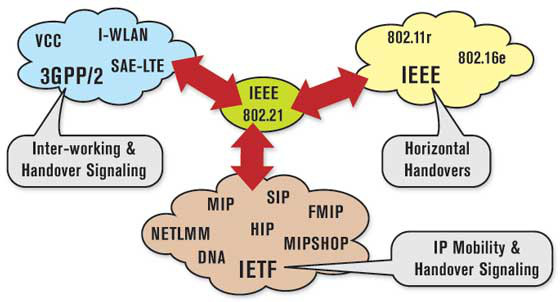
\includegraphics[scale=0.6]{ieee80221_cloud.jpg}
\caption{Rapporto con gli altri standards}
\label{fig:rapporto}
\end{figure}

\section{Architettura}
Lo standard IEEE 802.21 definisce più entità, rappresentate graficamente in figura \ref{fig:80221arch}, ognuna con il proprio specifico compito, al fine di fornire tutti i servizi necessari a prendere decisioni di {\em handover} in modo {\em media-independent}, ovvero in modo indipendente dalla tecnologia utilizzata in quel preciso momento:
\begin{itemize}
\item MIHF: implementa il core delle funzionalità offerte dallo standard.
\item MIH-SAP: fornisce una astrazione {\em media-independent} per tutti i tipi di interfacce.
\item MIH-LINK-SAP: fornisce una astrazione {\em media-specific} per una singola tecnologia.
\item MIH-NET-SAP: permette la gestione di MIHF remoti.
\item MIH-User: è l'entità che si sottoscrive ad un MIHF per usufruire dei servizi offerti.
\end{itemize}

\begin{figure}[h!]
\centering
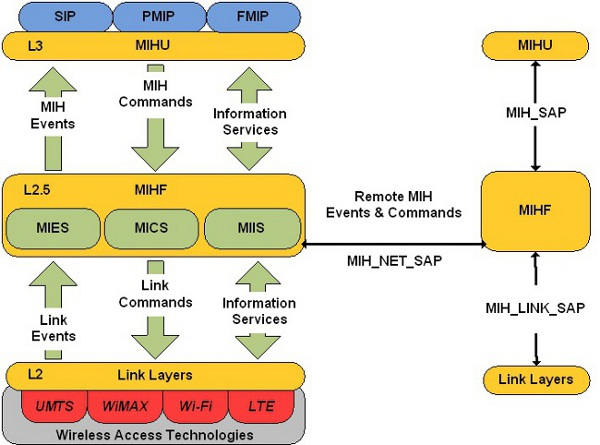
\includegraphics[scale=0.9]{ieee80221.jpg}
\caption{Architettura IEEE 802.21}
\label{fig:80221arch}
\end{figure}
\subsection{MIHF}
Questo componente è il più importante: i nodi mobili devono sottoscriversi ad un MIHF, il quale invierà loro una conferma con informazioni sui collegamenti disponibili, come i rispettivi indirizzi di livello due ed il tipo di tecnologia, ed un elenco di eventi e comandi supportati. Ogni MIHF fornisce un insieme di servizi astratti ai livelli superiori indipendentemente dalle tecnologie adottate dalle singole interfacce gestite.
L'implementazione della Media Independent Handover Function è formata da tre sottocomponenti:

\begin{itemize}
\item MIES (Media Independent Event Services): ha il compito di propagare gli eventi a tutte le parti interessate, come eventuali cambiamenti dello stato a livello {\em data link} agli strati superiori dello stack di rete del sistema locale o di sistemi remoti. Per un elenco completo di tutti gli eventi specificati nello standard IEEE 802.21 ed i loro significati si faccia riferimento alla tabella \ref{mihevents}. Gli eventi possono essere generati dall'MIHF stesso oppure dai livelli sottostanti. Il flusso dei dati generati da questo componente ha quindi un verso prettamente {\em bottom-up}.

\begin{table}[h]
\begin{tabular}{p{0.35\textwidth}|p{0.65\textwidth}}
\toprule
\textbf{Nome} & \textbf{Descrizione} \\
\midrule
Link\_Up & è generato quando una specifica interfaccia diventa attiva, i.e. viene stabilita una connessione di secondo livello\\
\hline
Link\_Down & è generato quando cade una connessione di secondo livello di una specifica interfaccia, e.g. disconnessione da una rete {\em wireless}\\
\hline
Link\_Detected & è generato quando è disponibile una nuova rete di cui usufruire, ad esempio la scoperta di una nuova rete {\em wireless} durante una scansione\\
\hline
Link\_Going\_Down & può essere generato da un SAP per informare le parti interessate che le prestazioni di un dato {\em link} stanno man mano degradando, secondo vari criteri, e.g. pacchetti persi, larghezza di banda, latenza, etc.\\
\hline
Link\_Handover\_Imminent & è utilizzato per comunicare alle entità interessate che sta per essere eseguita una procedura di {\em handover} \\
\hline
Link\_Handover\_Complete & è utilizzato per segnalare alle entità interessate che la procedura di {\em handover} è stata completata con successo\\
\bottomrule
\end{tabular}
\caption{Lista degli eventi specificati nello standard}
\label{mihevents}
\end{table}

\item MICS (Media Independent Command Services): è incaricato di propagare i comandi ricevuti dagli strati più alti dello stack di rete verso il basso per aiutare il nodo mobile ad eseguire più facilmente procedure di {\em handover}, ad esempio una richiesta esplicita di riconfigurazione per un'interfaccia, per comunicare ad un MIHF remoto di procedere con l'esecuzione di un {\em handover} oppure una richiesta di informazioni più dettagliate sullo stato di un collegamento specifico, e.g. richiedere il valore RSSI di un'interfaccia wireless. Per una lista completa di tutti i comandi previsti dallo standard IEEE 802.21 si faccia riferimento alla tabella \ref{mihcommands}. I comandi possono essere originati sia dall'MIH-User, sia dall'MIHF stesso. La destinazione dei comandi può essere per i livelli inferiori dello stack locale oppure di uno stack remoto, propagando il comando al peer MIHF appropriato. Il flusso dei dati è prettamente {\em top-down}.

\item MIIS (Media Independent Information Services): è la componente incaricata di gestire richieste di informazioni e la riconsegna delle opportune risposte. Ad esempio, un nodo mobile può essere interessato ad informazioni aggiuntive riguardo uno specifico {\em link}, come l'RSSI di una interfaccia 802.11, inviando una richiesta all'MIHF a cui è sottoscritto tramite il MICS ed aspettando una risposta dall'MIIS. Lo scambio di informazioni è effettuato secondo un modello RDF\footnote{Resource Description Framework} basato su XML\footnote{Extensible Markup Language}, variants\footnote{tipi varianti, e.g. boost::variant \cite{variants}} oppure TLV\footnote{Type-length-value}. In questo caso non è possibile stabilire un verso per il flusso delle informazioni, poiché uno strato superiore dello stack potrebbe richiedere informazioni circa un {\em layer} sottostante e viceversa.
\end{itemize}

\subsection{SAPs}
Questo componente è incaricato di interagire direttamente con le interfacce di rete, al fine di esporre dei servizi di basso livello di una singola interfaccia ad un MIHF, al quale deve essersi preventivamente registrato.
I Service Access Points possono essere di due tipi: {\em media-independent} e {\em media-specific}.
I primi forniscono servizi astratti per tutte le possibili tipologie di interfacce di rete, come la generazione di eventi {\em link\_down} e {\em link\_up}, e, di conseguenza, offrono un minor numero di servizi.
I secondi forniscono servizi specifici per una singola tecnologia, e.g. IEEE 802.3 od IEEE 802.11, e, per questo motivo, sono più espressivi dei primi: ad esempio, in seguito ad una richiesta {\em get\_link\_parameter} è naturale aspettarsi risposte differenti per ogni famiglia di tecnologie, come il valore dell'intensità del segnale che assume valori differenti a seconda della tipologia dell'interfaccia interrogata. 

\begin{table}[h]
\begin{tabular}{p{0.37\textwidth}|p{0.63\textwidth}}
\toprule
\textbf{Nome} & \textbf{Descrizione} \\
\midrule
Link\_Get\_Parameters & permette di richiedere informazioni aggiuntive riguardo un collegamento specifico \\
\hline
Link\_Configure\_Thresholds & permette di definire dei valori-soglia che facciano scattare degli eventi  \\
\hline
Link\_Capability\_Discover & permettere di ottenere la lista di eventi e comandi supportati da un MIHF  \\
\hline
Link\_Event\_Subscribe & permettere di registrarsi per essere avvisati di cambiamenti di stato di una particolare interfaccia\\
\hline
Link\_Event\_Unsubscribe & permette di rescindere la sottoscrizione effettuata con il comando precedente\\
\hline
Link\_Actions & permette di comandare esplicitamente l'interfaccia (e.g. {\em power\_up}, {\em power\_down}) \\
\hline
Net\_Ho\_Candidate\_Query & in {\em handovers} iniziati dalla rete, segnala al nodo mobile di procedere al passaggio ad uno dei network candidati \\
\hline
Net\_Ho\_Commit & conferma all'esecuzione dell'{\em handover} \\
\hline
N2n\_Ho\_Query\_Resources & prima di confermare l'esecuzione dell'{\em handover} su un altro network, l'attuale PoS contatta il candidato per controllare che abbia le risorse per accettare un nuovo nodo mobile \\
\hline
N2n\_Ho\_Commit & il passaggio verso il nuovo PoS è confermato\\
\hline
N2n\_Ho\_Complete & la procedura di {\em handover} è stata completata \\
\hline
Mn\_Ho\_Candidate\_Query & in {\em handovers} iniziati dal nodo mobile, serve per richiedere la lista dei network candidati per un eventuale passaggio \\
\hline
Mn\_Ho\_Commit & la procedura di {\em handover} è stata confermata \\
\hline
Mn\_Ho\_Complete & la procedura di {\em handover} è stata completata \\
\bottomrule
\end{tabular}
\caption{Lista dei comandi specificati nello standard}
\label{mihcommands}
\end{table}

\subsection{MIH-User}
L'applicazione a livello utente che si sottoscrive ad un MIHF è definita come MIH-User. Essa invia una richiesta di {\em capability\_discover} e riceve come risposta una lista di interfacce, eventi e comandi disponibili. Una volta ricevuto questo messaggio, l'applicazione deciderà a quali interfacce è interessata ed invierà di conseguenza una richiesta di sottoscrizione per ogni interfaccia scelta. In seguito essa potrà ricevere tutti gli eventi generati dal cambio di stato di ogni collegamento a cui si è sottoscritta ed inviare richieste e comandi al proprio MIHF, il quale si preoccuperà di interagire a sua volta con i SAPs che gestiscono le interfacce interpellate.

\section{Eventi e comandi}
Lo standard IEEE 802.21 specifica una serie di eventi e di comandi per gestire tutta la fase preparatoria dell'{\em handover}. Gli eventi definiti, riassunti in tabella \ref{mihevents}, servono a notificare alle entità interessate cambiamenti nello stato dei collegamenti disponibili e sono i seguenti:
\begin{itemize}
\item Link\_Up: viene generato da un SAP quando l'interfaccia gestita da esso stabilisce una connessione di livello {\em data link}, segnalando la corretta connessione ad un {\em access point}.
\item Link\_Down: viene generato da un SAP quando la connessione instaurata attraverso l'interfaccia gestita viene interrotta, ovvero quando non è più attivo il collegamento con l'{\em access point}.
\item Link\_Detected: è generato quando è disponibile un nuovo {\em access point} di cui poter usufruire attraverso una propria interfaccia, ad esempio la scoperta di una nuova rete {\em wireless} durante una scansione.
\item Link\_Going\_Down: può essere generato quando una particolare interfaccia sta per perdere contatto con il proprio {\em access point}, in modo da avvisare preventivamente l'MIH-User e consentire una gestione dell'{\em handover} prima che la connessione cada effettivamente. I {\em triggers} che fanno scattare la generazione da parte di un SAP di questo evento sono diversi per ogni tecnologia gestita, a seconda delle caratteristiche intrinseche del mezzo trasmissivo, ad esempio valori minimi per l'RSSI, percentuale di pacchetti persi, etc.
\item Link\_Handover\_Imminent: è utilizzato per comunicare a tutte le entità interessate che sta per essere eseguita una procedura di {\em handover} e, quindi, di prepararsi all'imminente passaggio.
\item Link\_Handover\_Complete: è utilizzato per segnalare alle entità interessate che la procedura di {\em handover} è stata completata con successo.
\end{itemize}

I comandi previsti dallo standard IEEE 802.21, raccolti in tabella \ref{mihcommands}, servono a richiedere informazioni aggiuntive su specifiche interfacce, gestirne lo stato e la loro riconfigurazione oppure per iniziare le procedure di {\em handover}. Nel dettaglio, i comandi previsti sono i seguenti:
\begin{itemize}
\item Link\_Get\_Parameters: permette di richiedere informazioni aggiuntive riguardo un collegamento specifico, come statistiche sui pacchetti persi, il {\em data rate} attuale, l'RSSI di interfacce wireless, etc.
\item Link\_Configure\_Thresholds: permette di definire dei valori-soglia che facciano scattare la generazione di {\em reports} sulle statistiche del collegamento per informare le entità interessate di eventuali cambiamenti nelle caratteristiche del {\em link}.
\item Link\_Capability\_Discover: permettere di ottenere la lista di eventi e comandi supportati da un MIHF, per consentire all'MIH-User di definire dinamicamente gli opportuni {\em callbacks} a seconda delle funzionalità implementate da ogni singolo MIHF.
\item Link\_Event\_Subscribe: permettere di sottoscriversi alla ricezione di eventi da parte dei SAPs richiesti per essere avvisati di eventuali cambiamenti di stato di una particolare interfaccia.
\item Link\_Event\_Unsubscribe: permette di rescindere la sottoscrizione effettuata con il comando precedente.
\item Link\_Actions: permette di comandare esplicitamente l'interfaccia, ad esempio è possibile accendere o spegnere fisicamente una ricetrasmittente a seconda del suo utilizzo, in modo da ottimizzare i consumi energetici quando non è in uso.
\item Net\_Ho\_Candidate\_Query: in {\em handovers} iniziati dalla rete, segnala al nodo mobile di procedere al passaggio. Nella richiesta è anche allegata una lista di {\em networks} candidati, ovvero un elenco di altre reti disponibili a cui il nodo mobile dovrà collegarsi.
\item Net\_Ho\_Commit: in {\em handovers} iniziati dalla rete, la ricezione di questo evento conferma l'esecuzione dell'{\em handover}, quindi il nodo mobile dovrà necessariamente procedere al passaggio ad un {\em network} comunicato precedentemente.
\item N2n\_Ho\_Query\_Resources: prima di confermare l'esecuzione del passaggio ad un altro network, l'attuale PoS\footnote{Point of Service} contatta quello candidato per controllare che abbia le risorse per accettare un nuovo nodo mobile. Se il nuovo PoS si dichiara disponibile a ricevere un nuovo nodo mobile, il passaggio sarà confermato attraverso un successivo {\em commit}.
\item N2n\_Ho\_Commit: il passaggio verso il nuovo PoS è confermato ed i nodi mobili devono provvedere all'esecuzione dell'{\em handover}.
\item N2n\_Ho\_Complete: la procedura di {\em handover} verso un nuovo PoS è stata completata.
\item Mn\_Ho\_Candidate\_Query: in {\em handovers} iniziati dal nodo mobile, serve per richiedere la lista dei network candidati per un eventuale passaggio.
\item Mn\_Ho\_Commit: in {\em handovers} iniziati dal nodo mobile, serve a comunicare che la procedura di {\em handover} è stata confermata.
\item Mn\_Ho\_Complete: in {\em handovers} iniziati dal nodo mobile, serve a comunicare che la procedura di {\em handover} è stata completata.
\end{itemize}

\section{Esempio d'uso}
Si supponga di disporre di un dispositivo mobile dotato di più interfacce di rete {\em wireless} e che sia connesso tramite una di queste. Esso potrebbe richiedere al proprio MIHF, al quale deve essersi precedentemente sottoscritto, informazioni su tutti i  collegamenti disponibili, indipendentemente dalla tipologia dell'interfaccia utilizzata in quel momento. In questo modo l'utente potrebbe venire a conoscenza preventivamente dell'esistenza di altri potenziali collegamenti tramite una differente tecnologia senza dover accendere fisicamente sul proprio dispositivo la ricetrasmittente appropriata per effettuare una scansione manuale, con un potenziale guadagno sui consumi energetici e maggior parsimonia per quanto riguarda lo sfruttamento dell'etere. Successivamente l'applicazione utente potrebbe essere informata di un deterioramento nelle prestazioni dell'interfaccia con la quale è attualmente connessa attraverso la ricezione dell'evento {\em Link\_Going\_Down} e quindi prepararsi ad azioni di {\em handover} richiedendo informazioni su altre reti disponibili con il comando {\em Mn\_Ho\_Candidate\_Query} al fine di designare il prossimo PoA\footnote{Point of Access} a cui collegarsi, confermando l'eventuale operazione di {\em handover} con un {\em commit} impartendo il comando {\em Mn\_Ho\_Commit} per informare il proprio MIHF dell'imminente passaggio. Una volta completato, l'MIH-User dovrà confermare il successo dell'operazione con il comando {\em Mn\_Ho\_Complete}. La situazione appena descritta è riferita ad un {\em handover} iniziato dal nodo mobile, ma può anche accadere che il passaggio sia richiesto dal proprio MIHF, in questo caso saranno utilizzati i comandi {\em Net\_Ho\_Commit} e {\em Net\_Ho\_Commit} per segnalare che l'operazione è richiesta dalla rete stessa: in questo caso l'MIHF invierà di propria iniziativa una lista di altri {\em networks} all'applicazione utente, richiedendo il trasferimento verso uno di essi. In questo modo l'MIH-User può recuperare tutte le informazioni utili per gestire le decisioni di {\em handover} in modo indipendente dalla tecnologia utilizzata per comunicare con il proprio MIHF e può, a questo punto, sfruttare questi dati per svariati compiti, come per implementare un proxy ad alta affidabilità oppure una sorta di {\em network manager} che di volta in volta si preoccupi di sottoscriversi ad ogni MIHF e di decidere l'interfaccia migliore secondo un {\em tradeoff} tra consumo energetico e qualità del segnale, sempre supponendo di aver a disposizione soluzioni di {\em IP mobility}.

\section{Stato dell'arte}
Attualmente è possibile testare lo standard in due modi: eseguendo una sua implementazione oppure simulandolo. La maggior parte della letteratura esistente si concentra su simulazioni all'interno di {\em ns-2}\cite{ns2} e {\em ns-3}\cite{ns3}. Queste simulazioni sono in grado di dimostrare come le funzionalità introdotte dallo standard possano essere utili per ridurre i tempi necessari per effettuare un {\em handover}\cite{master}, in particolare per quanto riguarda la scelta del nuovo {\em network}, grazie all'MIIS che permette di conoscere le reti disponibili senza dover far uno {\em scan} esplicito. Per quanto riguarda le implementazioni realmente eseguibili, la più utilizzata e studiata è ODTONE\cite{odtone}, la quale sarà analizzata nel dettaglio nel prossimo capitolo.